\documentclass[letterpaper,twocolumn,11pt]{article}
%\usepackage{fontspec}
%\setmainfont[
%   ItalicFont     = HelveticaNeue-Italic,
%   BoldFont       = HelveticaNeue-Bold,
%   BoldItalicFont = HelveticaNeue-BoldItalic]{HelveticaNeue}
\usepackage{epsfig,endnotes,usenix}
\usepackage{lastpage}
\usepackage{titling}
\usepackage[hyphens]{url}
\usepackage{graphicx}
\usepackage[TABBOTCAP]{subfigure}
\usepackage{pslatex}
\usepackage{amsmath}
\usepackage[noend]{algpseudocode}
\usepackage{xspace}
\usepackage[normalem]{ulem}
\usepackage[table]{xcolor}
\usepackage[pdftex,bookmarks=false,colorlinks=true,citecolor=blue,filecolor=black,linkcolor=blue,urlcolor=black]{hyperref}
\renewcommand*{\sectionautorefname}{Section}
\DeclareGraphicsExtensions{.eps,.jpg,.png,.gif}
\graphicspath{{./images/}}
\usepackage{color}
\usepackage{ifpdf}
\usepackage{enumitem}
\usepackage[font=footnotesize,labelfont=bf,skip=5pt]{caption}
\usepackage{tabulary}
\usepackage{relsize}
\usepackage{amsmath}
\usepackage{pifont}
\usepackage{multirow}
\usepackage{booktabs}
\usepackage{pbox}
\usepackage[square,comma,numbers,sort&compress]{natbib}


\author{\rm Haichen Shen\\ 
       haichen@cs.washington.edu \\
       University of Washington \\
       }
\date{}


\begin{document}

\title{Using Database to Model Internet Topology}
\maketitle

\section{Introduction}

%Our world is full of all diversed networks, ranging from social networks to collaboration networks, from road networks to the Internet networks, etc. Each network can be regarded as a graph-oriented dataset. Nowadays, these graph datasets are usually very large, up to thousands or tens of thousands of nodes, and up to millions of edges. Moreover, the size of graph keeps growing with the lapse of time. For instance, in 2010, Facebook has 608 million active users, while this number becomes 1.23 billion by 2013 \cite{fb_users}. A measurement study \cite{ager2012anatomy} shows that the Internet consisted of at least half a million peering links between distinct ASes in 2011. Hence, how to store, manage, and query a large graph becomes a much more challenging task.

The Internet is an enormous global interconnected network that contains thousands of {\it Autonomous Systems} (AS) ranging from regional or international service providers, content providers, enterprise and academic networks, and exchange points. Because of its complexity and variety, it makes Internet measurement and reasoning a hard problem for researchers. However, understanding the topology of Internet and its evolution is substantially beneficial in many aspects, such as troubleshooting the slow connections and network outages, selecting a route with lower latency and higher bandwidth, and even help with developing a better routing algorithm.

The difficulty of modeling Internet topology mainly comes from three aspects: (a) The entire Internet topology is large and complex. Apart from great amounts of nodes and edges, the Internet also appears as a different graph when looking at different level of granularity. (b) Data sources are heterogeneous. Researchers develop many methods to measure and monitor the Internet. For example, the BGP table snapshots provides the information of the IP prefixes to AS mapping and peering AS links. Traceroute reveals the actual links from one location to another throughout the Internet, albeit in a distinct form of data. (c) Internet is not static. In fact, study \cite{zegura1997quantitative} \cite{edwards2012internet} show the topology keeps evolving from time to time. Therefore, it is necessary to manage the data from a range of days, months, or even years, in order to fully analyze the Internet topology.

In consideration of the above difficulties, storing the Internet topology related data into a database is favorable. The data model of Internet topology is simply a graph. It consists of nodes and edges, where each node and edge associates with certain data. Edges can be either directed or indirect. In addition, this graph also evolves over the time, meaning that a node or an edge might exist in the graph at one time but not exist at another time. The workload for such a database includes (a) getting information of nodes and edges, (b) filtering and ordering nodes according to the degree, (c) finding (shortest) paths between nodes.

To manage such type of data, we actually have many choices in the database models. In this project I only consider two types of databases, relational databases and graph databases. Relational databases are the dominating model in this era. Graph databases, which are designed to store and manage graphs, emerge recently, along with the popularization of NoSQL databases. Using the relational databases, a graph can be simply organized in two tables, one for the nodes and its associated data, the other for the edges. For graph databases, it's straightforward for the data schema, since graph databases inherently support the notion of nodes and edges. 

However, it is unclear which type of database model performs better in executing queries over a graph. 
Since the underlying models are different between relational databases and graph databases, the query language, supported functionality, and corresponding optimizers of these two can be divergent. As a consequent, the performance of executing the same queries varies. 
In this project, I explored and compared the performance of three types of workload mentioned above between relational database and graph database. Given that graph databases support queries that are not supported in traditional SQL queries, e.g., finding path, I implemented the algorithm while using SQL queries to access data.

In this project, I selected MySQL \cite{mysql} for the relational database and the Neo4j \cite{neo4j} for the graph database. I built a front end system that can predict the network routes between arbitrary IP addresses. The system can use either Neo4j or MySQL as its back end database system. 
%Both databases are popular, modern and open-sourced databases. Their performance comparison should be a good indicator to find out which type of database model suits better for a large graph dataset. The graph dataset used in the evaluation is the Internet measurement results. In this measurement, over 200 nodes issued traceroutes to 78,744 targets all over the world and recorded all hops in each traceroute. Later I converted the traceroute results into a graph with undirected edges. The graph consists of XXX nodes and XXXX edges. The measurement carried out for XX days, which allows me to issue queries about the changes in the graph over the time.

The evaluation results show that MySQL and Neo4j has similar performance in simple queries. MySQL executes traditional SQL analytic queries faster than Neo4j does. However, to accomplish same task, the SQL query is much more complicated to express than Cypher query, the query language used by Neo4j. Furthermore, MySQL is worse than Neo4j in finding the shortest path between two nodes.

In section 2, I will introduce the graph database model used by Neo4j and query language devised for querying a graph. Section 3 explains how the data set is collected and converted into a graph. Section 4 provides a step by step overview of how the data is stored in both MySQL and Neo4j database, and the testing queries issued to them. Evaluation results are shown in the Section 5.

\section{Background}
\label{sec:background}
In this section, I will give a brief introduction to the concept of graph databases and the query language adopted by Neo4j for graph analytic. 

\subsection{Graph Databases}
Graph databases is a nominal name for graph-oriented databases. They are usually categorized in the NOSQL databases, but somehow different from NOSQL databases. Graph databases can be further classified into two parts based on their design purpose: {\it online graph analytic} and {\it offline graph processing}. Graph databases designed for online graph analytic aim to reduce the query execution time so that it can be accessed from an application in real time. Yet graph databases designed for offline processing focus on graph compute engines that can processed and analyzed data in a large scale. They are mostly used for data mining and big data processing. In this paper, we only focus on graph databases for online analytic.

There are two major features that can distinguish the graph databases from relational databases: the underlying storage and the processing engine.

\paragraph{Underlying Storage} There is no universal storage strategy for graph databases. Some graph databases use {\it native graph storage} which inherently supports and optimizes for all graph models, e.g. Neo4j \cite{van2014learning}. The fundamental building blocks of native graph storage contain
\begin{itemize}
\item {\bf Nodes}: These are used to store the entity information.
\item {\bf Relationships}: These are the connection linked from one node to one another, as a means of constructing the graph.
\end{itemize}
Besides the above two building blocks, others such as properties and labels of nodes and relationships also come with graph databases.

However, some other graph databases construct and serialize the graph data into a relational database, and optimizes the processing engine to improve the performance for graph related queries, e.g. Vertexica \cite{jindal2014vertexica}. Besides, object-oriented databases and some other general-purpose data stores are used for graph analytic as well.

\paragraph{Processing Engine} A major difference between SQL query and graph query is that graph query often performs at a global scale. Usually a graph query may need to visit every table in the database to finish. It indicates in relational database that a query involves many join operations in between tables. Furthermore, a query that traverses a graph may cause numerous relational queries to a same table. As a result, the processing engines of graph databases primarily optimize the performance for traversing through graphs.

Graph databases with native graph storage can traverse from one node to another without involving expensive table joins. Graph database with relational storage, for example, Vertexica \cite{jindal2014vertexica}, unions the table together to avoid join operation. It also use parallel workers, vertex batching, and some other techniques to accelerate the query processing. Nevertheless FlockDB \cite{flockdb}, the graph database developed by Twitter, limits the graph model only supporting single-depth followers/following in exchange for latency.

\subsection{Query Language: Cypher}
Cypher is a new query language designed by Neo4j for graph query. Complicated database queries become more easily to read and understand in the expression of Cypher.

Neo4j doesn't require to create a data schema in advance. Instead, one can specify the entities and relations during the data insertion. Each entity and relation can have both labels and properties, which properties are key-value pairs. Both entity and relation can have infinite properties. Entity can have more than one labels, while relation can only be assigned by one label currently. For example, 
\autoref{fig:example} can be expressed in \\
{\small
\texttt{(a:USER \{name:'Peter'\}),
\texttt{(a:USER)-[:KNOWS]->(b:USER)-[:KNOWS]->(c:USER)}, \\
\texttt{(a:USER)-[:KNOWS]->(c:USER)}, \\
}
where \texttt{(n:LABEL \{}\textit{properties}\texttt{\})} refers to a node, and \texttt{-[:LABEL]->} refers to a relation from one node to another.

\begin{figure}[t]
\centering
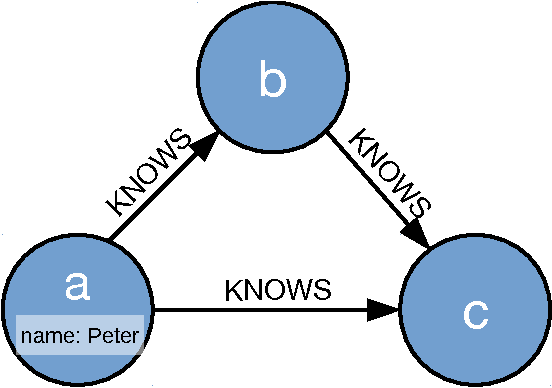
\includegraphics[height=4cm]{figs/example.pdf}
\caption{A simple graph example}
\label{fig:example}
\end{figure}

Cypher uses \texttt{MATCH} to specify a pattern to match nodes, relations, or both at the same time. For instance, you can match the user whose name is Peter by \texttt{MATCH (n:USER \{name:'Peter'\})}. To match the users who know Peter, query is written as \texttt{MATCH (a:USER)-[:KNOWS]->(b:USER \{name:'Peter'\})}.

The key word \texttt{RETURN} in Cypher is similar to \texttt{SELECT} in SQL query. It specifies the returned data of which nodes, relationships, and properties in the matched data to the client. \texttt{CREATE} is used to insert data into the database. Other clauses such as \texttt{WHERE}, \texttt{DELETE}, \texttt{WITH}, etc., are also included in the Cypher query language.

\section{Data set}

Since the Internet is such an enormous interconnected system, we need to decide at which level that we want to model it. It is impractical that we model the Internet at the finest granularity, the IP level. There are over 4 billion different addresses in the whole IPv4 address spaces, not even to mention more links between IPv4 addresses and the gradually popularizing IPv6 addresses, which can contain exponentially more addresses than IPv4 in theory. Therefore, we need to cluster IP addresses into a high-level concept that can be used to model the Internet. 

An {\it autonomous system} (AS) is an Internet entity that controls a collection of connected IP prefixes. IP prefixes within a single AS presents the same routing policy to the rest of the Internet. In other words, one from outside an AS cannot tell the difference in terms of routing paths among the IP prefixes belonging to this AS. Each AS is assigned to a unique {\it autonomous system number} (ASN). For example, AS73 is under charge of University Washington. AS73 contains the following IP prefixes set.

\hspace{8pt}
\fbox{
\begin{minipage}[t]{0.4\linewidth}
108.179.128.0/18 \\
198.48.64.0/19 \\
205.175.96.0/19 \\
173.250.128.0/17 \\
198.48.92.0/22 \\
69.91.128.0/17 \\
140.142.0.0/16 \\
128.208.0.0/16 \\
128.95.0.0/16
\end{minipage}
}
\vspace{6pt} \\ 
These properties of AS allows us to cluster IP addresses into ASes, and significantly reduce the size of the graph. and treat an AS as a simple node in the Internet topology.

As a result, our data sets for modeling the Internet topology contain three types of data: (a) IP prefixes to ASN mapping, (b) ASN and AS description, (c) AS links.

\subsection{IP Prefixes to ASN}
This data set contains 624,342 records from IP prefixes to ASN mapping. The data is collected from RouteView \cite{routeview}, which collects the BGP table snapshot. We then extracted the IP prefixes to ASN mapping from BGP table. With this mapping data set, for any arbitrary IP address, we can first find the IP prefix that contains it, and then map from the IP prefix to an ASN. However, due to the amount of records is still a large number, I didn't insert the data into either of the database. Otherwise, it will take a long time till the insertion finishes. Instead, I ran a C program that mapped the IP address to a corresponding ASN.
\subsection{ASN and AS Description}
This data set contains a list of ASes data, including ASN and description. The data is downloaded from CIDR report website \cite{cidr} \cite{cidr-website}. It contains 72,934 rows of ASNs and AS descriptions. These data will later be inserted as node data into the database.

\subsection{AS Links}
AS links construct the edges between AS nodes. This data comes from a collection of measurement results. Measurement is carried out on the PlanetLab platform \cite{chun2003planetlab}. PlanetLab is a global overlay network that allows researchers to deploy and test broad-coverage services. We issued traceroutes every day on about 180 geo-distributed nodes targeting to 78.7k different IP addresses over the Internet. The target IP list is picked one ping-able IP address per AS so that we can maximize the exploration of Internet topology with a smallest target list. The traceroutes reveal about 85k AS links in one day. The data is stored into database associated with date.


%Given that Internet consists of various different components, we need to gather the measurement results from multiple sources including online public data sources and measurements committed by ourselves. These data sets are usually in heterogeneous formats, defective, repeated, and sometimes even contradictory. How to store, manage, and further analyze these data in a database is a key challenge in this project. In addition, Internet topology is never constant; instead it changes quite frequently. Comparisons of measurement results between epochs and between different vantage points are inevitable and favorable for reasoning the topology transitions.

%The purpose of this measurement is to figure out the connectivity among all ASes. The measurement consists of over 200 probing servers sending traceroute packets to the destination IP addresses throughout the Internet. These probing servers belong to Planetlab platform \cite{madhyastha2006iplane}. Planetlab is a global overlay network that allows researchers to deploy and test broad-coverage services, including the measurement of the Internet at a large scale. It contains 1343 nodes at 657 geographically distributed sites all over the world. 

%I am going to use three online public datasets and collect traceroute measurements from about 30 different places for the entire analysis. The three online public data sets are (a) IP address to AS number mapping from RouteView [1] project, (b) Internet exchange point (IXP) data from PeeringDB [2], (c) iPlane \cite{madhyastha2006iplane} daily traceroute data, based on PlanetLab platform \cite{chun2003planetlab} Our measurement runs daily from 30 Yahoo CDN PoPs, tracerouting to about 10.7M targets. The results is expected to disclose the Internet topology changes from day to day, and difference in topology seen from Internet core and seen from Internet edge.

\section{Approach}
In this section, I will first show how I set up the the database, inserted the data into database. Then I will introduce the query front end for predicting paths between two arbitrary IP addresses.

\subsection{Database Setup and Insertion}
I created two tables in MySQL database. The first table called \texttt{astable} stores AS information. It contains two fields, \texttt{asn} and \texttt{description}, where \texttt{asn} is unique and acts as primary key for this table. The corresponding SQL query is
\begin{quote}
\texttt{CREATE TABLE astable (asn int not null, description text);}
\end{quote}

The second table \texttt{aslink} stores the daily AS links information. It contains three fields, \texttt{asn1}, \texttt{asn2}, and \texttt{date}, where \texttt{asn1} and \texttt{asn2} are foreign keys from table {\tt astable}. The corresponding SQL query is
\begin{quote}
{\tt
CREATE TABLE aslink (\\
\-\ \ \ \ asn1 int not null, \\
\-\ \ \ \ asn2 int not null, \\
\-\ \ \ \ date DATE);
}
\end{quote}

After the initial insertion to both tables, I created two index keys, \texttt{asn} for table {\tt astable} and Pair {\tt (asn1, asn2)} for table {\tt aslink}.

The initialization of Neo4j works quite differently, since Neo4j doesn't require the data schema. Each node or entity stores the AS information, whereas the edges or relations store the AS link information. I first insert the node by running Cypher query
\begin{quote}
{\tt CREATE (:AS \{asn:{\it asn}, desc:'{\it desc}'\});}
\end{quote}
Next, I insert daily links between nodes by running the query
\begin{quote}
{\tt MATCH (as1:AS \{asn:{\it asn1}\}),\\
\-~~~~~~(as2:AS \{asn:{\it asn2}\}) \\
CREATE (as1)-[:Date{\it date}]->(as2);}
\end{quote}
Note that I set the {\it date} as an edge label, rather than a property of an edge. This is due to the constraint of Neo4j that the {\tt WHERE} clause can be only applied to edge label not to edge property. 

An caveat I learned in this project is that before the insertion of relations, it is necessary to create an index for the entities. Otherwise, the insertion of relations without an index is much slower than that with an index. In my case, if I didn't create the index for AS nodes, the insertion of one-day links (about 85k records) took about 8.3 hours. However, after I created the index, the insertion time reduced to merely 0.8 hours. It is about the same time of insertion in MySQL.

\subsection{Query Front-end}

I built a query front-end system for path prediction between two arbitrary IP addresses. The system takes two IP addresses as input, and outputs one or all shortest path(s) from one IP address to the other. \autoref{fig:front-end} exhibits an overview of the front-end system. The front-end system provides the options to connect to either MySQL database or Neo4j database as the back end data storage. 

\begin{figure}[t]
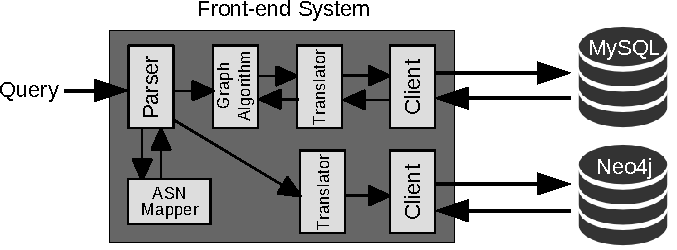
\includegraphics[width=\linewidth]{figs/front_end.pdf}
\caption{Overview of the front-end system}
\label{fig:front-end}
\end{figure}

The front-end system supports an command-line interface (CLI) for user to input the request. The format of request is 
\vspace{6pt}\\
\-\hspace{15pt}
{\tt from {\it ip\_addr1} to {\it ip\_addr2} (on {\it date}) (all)}
\vspace{6pt}\\
where {\tt on} {\it date} and {\tt all} are optional. Option {\tt on} {\it date} allows user to query the path on a particular day. Option {\tt all} returns all possible paths from {\it ip\_addr1} to {\it ip\_addr2}.

After user submits the request, a parser will parse the request and extract required data. During the parsing, the parser converts the IP addresses to ASNs that control these IP addresses by connecting to the ASN Mapper which maps the IP address to an ASN. The rest of the system only uses ASN to search the shortest paths. 

Based on the back end user connects to, the parser passes the request to different parts. Since Neo4j itself supports searching one or all shortest path(s) functions, if user connects to Neo4j, the system only needs to pass the request to the translator for Neo4j which translates the request to Cypher query language. The query used for searching one shortest path on a specific date is \vspace{2pt}\\
%\begin{quote}
\fbox{
\begin{minipage}{0.94\linewidth}
{\tt
MATCH (s:AS \{asn:{\it asn1}\}),(d:AS \{asn:{\it asn2}\}), \\                                  
\-~~paths=shortestPath(s-[:Date{\it date}*]-d) \\
\-~~RETURN NODES(paths);
}
\end{minipage}
} \vspace{2pt}\\
After the actual query is generated, a client sends the request to Neo4j database and retrieves the result from it.

However, MySQL doesn't have any functions for searching shortest paths. Therefore, we need to implement the algorithm in our front-end system. I implemented a {\it breath-first search} (BFS) algorithm in the system to complement the deficient support from MySQL. When the algorithm needs to access to the data, it sends a query through the translator and client delegate to retrieve the data from MySQL database. The query for searching all neighbors of one AS is (if considering the edge is indirect) \vspace{2pt}\\
\fbox{
\begin{minipage}{0.94\linewidth}
{\tt
SELECT asn2 from aslink where asn1={\it asn};\\
SELECT asn1 from aslink where asn2={\it asn};
}
\end{minipage}
} \vspace{2pt}\\
After the algorithm finishes, the system returns the result to user. 

The front-end system is implemented in Ruby language. It integrated the vanilla Ruby client from the developers of MySQL and Neo4j to connect to both databases. So the overhead introduced by Ruby client should be negligible. 

\section{Evaluation}
Three types of workload listed below are tested in this project. These workload reveals a real case usage in practical. It covers most of analytic that researcher wants to know about the Internet topology.
\begin{enumerate}
\item Node and edge information query,
\item Ranking AS nodes to tiers according to its connectivity,
\item Predicting routes between arbitrary IP addresses.
\end{enumerate}

I compared the performance of both databases on every workload, and also evaluated the complexity of query to accomplish the job.

\subsection{Results}

\paragraph{Node Information Query}

This task is the simplest one. I tested the query time to get AS description from an ASN for both databases. The queries used in the evaluation are listed below.
\begin{center}
\fbox{
\begin{minipage}{0.94\linewidth}
MySQL\\
{\tt
SELECT description FROM astable WHERE asn=73;
}
\end{minipage}
}\\
\vspace{6pt}
\fbox{
\begin{minipage}{0.94\linewidth}
Neo4j\\
{\tt
MATCH (n:AS {asn:73}) RETURN n.desc;
}
\end{minipage}
}
\end{center}

Query time is shown in \autoref{tab:performance}. We can see that both databases finish this query within 0.1 second. Neo4j appears a little bit faster than MySQL in this task. Both query expression is simple and easy to understand.

\begin{table}
\begin{tabular}{ccc}
\hline
{\bf Task} & {\bf MySQL (sec)} & {\bf Neo4j (sec)}\\
\hline
Node Information & 0.08 & 0.023 \\
Ranking & 0.38 & 0.779 \\
\hline
\end{tabular}
\caption{Query time of node information and ranking AS nodes for MySQL and Neo4j.}
\label{tab:performance}
\end{table}

\paragraph{Ranking AS Nodes} Researchers usually rank the ASes into tiers according to its connectivity to the entire Internet. For example, if an AS has links to more than 800 ASes, it is categorized as Tier-1 AS. This task can be converted into the following queries in MySQL and Neo4j.
\begin{center}
\fbox{
\begin{minipage}{0.94\linewidth}
MySQL\\
{\tt
SELECT description, degree\\
\-~~FROM astable JOIN (\\
\-~~~~SELECT asn1, count(*) as deg \\
\-~~~~FROM aslink\\
\-~~~~WHERE date='2015-02-19' \\
\-~~~~GROUP BY asn1 \\
\-~~~~HAVING deg >= 800) AS tmp \\
\-~~ON astable.asn = tmp.asn1 \\
\-~~ORDER BY deg DESC;
}
\end{minipage}
}\\
\vspace{6pt}
\fbox{
\begin{minipage}{0.94\linewidth}
Neo4j\\
{\tt
MATCH (n:AS)-[:Date20150219]->(:AS) \\
\-~~WITH n, count(*) AS degree \\
\-~~WHERE degree >= 800\\
\-~~RETURN n.desc, degree\\
\-~~ORDER BY degree DESC;
}
\end{minipage}
}
\end{center}

From \autoref{tab:performance}, MySQL completes this query faster than Neo4j does. However, the SQL query to MySQL database is much more complicated than the query to Neo4j, even nested with a inner query. The SQL query is harder to write and understand, and prone to be erroneous, though the performance of MySQL is better.

\paragraph{Route Prediction} Route prediction has the widest usage in Internet topology modeling. It allows the researchers to understand the traffic routes throughout the Internet and diagnose any problems in Internet. Presumably a route prediction system can receive a great amount of requests. Query time of searching shortest paths determines how many requests the system can handle in a time.

I tested my front-end system with different IP address pairs. I found the performance varying due to the different pairs. For example, to find a shortest path from 128.208.4.1 (University of Washington) to 8.8.8.8 (Google), Neo4j takes 0.021 seconds to return the result, while MySQL takes 1.172 seconds. However, searching the shortest path from 8.8.8.8 to 128.208.4.1 takes Neo4j 0.009 second and MySQL 853.9 seconds. We see a huge performance contrast for MySQL to find the shortest path. The reason is because the former request only incurs 22 queries to MySQL, whereas the latter request incurs about 21k queries. Whenever the path traverses a node with a huge fan-out, the total number of queries required for MySQL increases accordingly. 

Overall, Neo4j has a much lower query computing time than MySQL does in route prediction task.

\subsection{Graphic Interface}

\begin{figure}[t]
\centering
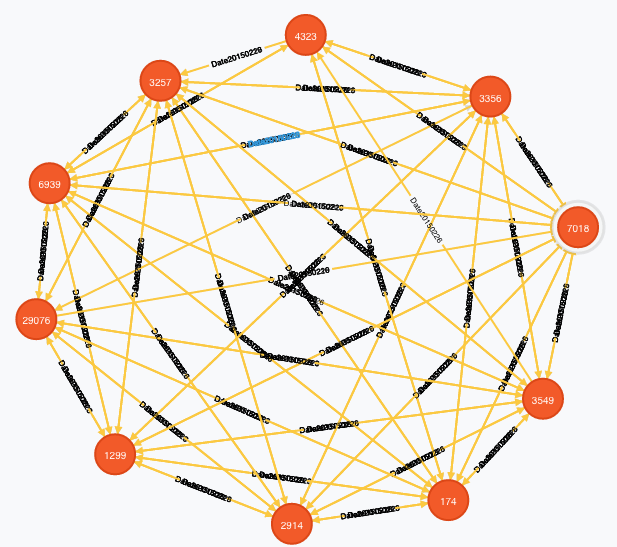
\includegraphics[height=5cm]{figs/gui.png}
\caption{Neo4j graphic interface}
\label{fig:gui}
\end{figure}

Neo4j has an exclusive feature, which is the graphic interface. It hosts a web site that allows user to query the database and displays the result in the web page if possible. \autoref{fig:gui} shows an example of graph results. This inherent graphic interface makes the result look more intuitive and easier to understand and analyze.

%\section{Discussion}

\section{Related Work}
Recently many systems focus on general graph processing and analytic. As we mentioned in \autoref{sec:background}, the graph processing can be categorized into online analytic and offline processing.

MapReduce \cite{dean2008mapreduce}, Spark \cite{zaharia2012resilient}, Pregel \cite{malewicz2010pregel}, GraphLab \cite{low2012distributed} all contribute to accelerate the offline graph processing. MapReduce provides a general platform with easy programming interface for parallel computing over large data sets and graphs. Spark optimizes MapReduce system by keeping all the temporary results in the main memory instead of expensive I/O operations. Its main application is for large data set iterative processing instead of real-time analytic. Pregel and GraphLab are designed for graph algorithms and processing. Pregel works in synchronous pipeline with message passing among machines, while GraphLab works asynchronously over a shared-memory model. A major characteristic for offline processing system is that they usually batches queries to reduce the overall computation time.

Vertexica \cite{jindal2014vertexica} explores how to make a relational database system friendly to graph analytic. To improve the graph traversing performance, it applies several optimizations such as table unions, parallel workers, and vertex batching. With the combination of these optimizations, Vertexica exhibits about 4x performance improvement on small graphs, and out-performs all other systems. 

Neo4j \cite{neo4j}, FlockDB \cite{flockdb}, OrientDB \cite{orientdb}, etc., belong to graph databases for online analytic. Neo4j is purely designed for graph analytic. OrientDB has a hybrid document-graph engine that adds some support to graph model. FlockDB is customized for Twitter usage case. It only supports limited shallow graph models.

Other researches such as \cite{vicknair2010comparison} compare performance between the graph databases and relational databases. It measures the query execution time over a series of different sizes of data sets. Their experiments show similar results as I did in this project.

%\section{Future Work}
%Difference between the graphs from two epochs.

\section{Conclusion}
In this project, I used the database to model the Internet topology. I collected and processed three different data sets from various sources and measurement results. I built a front end system that can predict the routes between two arbitrary IP addresses. I picked MySQL and Neo4j to compare the performance of three different types of workload. The results show that Neo4j is much faster in traversing graphs and finding shortest paths, while about same or a little bit slower than MySQL in relational queries.

\bibliographystyle{abbrv}
{
%\small
\bibliography{ref}  % ref.bib
}

\end{document}